\documentclass[a4paper]{article}
\usepackage[a4paper, total={6in, 9in}]{geometry}
\usepackage[T1]{fontenc}
\usepackage{bookman}
\usepackage{amsmath}
\usepackage{csvsimple}
\usepackage{graphicx}
\usepackage{siunitx}
\usepackage{float}
\usepackage{subcaption}
\usepackage{blindtext}
\usepackage{mathtools}
\usepackage[hidelinks]{hyperref}
\usepackage[style=iso]{datetime2}
\usepackage[shortlabels]{enumitem}
\usepackage{hyperref}

\graphicspath{ {./img/} }

\title{Summary of the Polarisation lab}

\author{Emil Babayev}
\date{\today}
\begin{document}
\begin{titlepage}
	\centering
	
\includegraphics[width=0.15\textwidth]{logo.png}\par\vspace{1cm}
	{\scshape\large Lunds Tekniska Högskola \par}
	\vspace{1cm}
    {\scshape\large FAFF30 Våglära och optik\par}
	\vspace{1.5cm}
	{\huge\bfseries Summary of the\\Polarisation lab\par}
	\vspace{2cm}
	{\Large Emil Babayev\par}
	\vfill
	Supervisor\par
    David Busto

    \vfill
    
	{\large \today \par}
\end{titlepage}
\section{Preparatory problems}
\subsubsection{Polarised light}
\begin{enumerate}[a)]
    \item The y-component is a cosine-wave, i.e. a sine wave shifted by $\pi/2$ rad, meaning the phase difference is $\pi/2$ rad. The light is circularly polarised.
    \item $cos(x) = sin(x + \pi/2)$ combined with the negative sign creates a phase shift of $\pi$ radians, giving linearly polarised light.
    \item The light is phase-shifted by $\pi/2$ but has different amplitudes, meaning it's elliptically polarised.
    \item There is a phase shift of $\pi/3$ rad, and the amplitudes are the same, meaning it's elliptically polarised.
\end{enumerate}

\subsubsection{The law of Malus}
The amplitude of the electric field passing through an ideal linear polariser is given by
\begin{equation*}
    E = E_0 cos(\theta)
\end{equation*}
where $\theta$ is the angle between the polariser and the linearly polarised light. Because the intensity is the square of the amplitude, this gives the intensity
\begin{equation*}
    I = E^2 = E_0^2 cos^2(\theta) = I_0 cos^2(\theta)
\end{equation*}
which is the law of Malus, giving the intensity of the light passing through the polariser.

\subsubsection{Birefringence}
Different materials have different internal structures. Light, which is electromagnetic radiation, oscillates the electrons in a material when propagating through it.
Glass, for example, is amorphous, and the atoms are randomly distributed. Light entering the glass approximately meets the same resistance to oscillation and therefore
has the same refractive index for all polarisations of light. 

Some materials (e.g crystals) are organised in such a way that it is harder to oscillate the electrons in
some directions than other. This means the same material has two different refractive indices depending on the polarisation of the incident light, and this is called birefringence
(sv. dubbelbrytning). 

If two axes are chosen, called the ordinary and the extraordinary axis, one may define two refraction indices for linearly polarised light incident on these
axes. If the refraction index along the ordinary axis is called $n_o$, and along the extraordinary axis $n_e$, the difference between refractive indices can be determined,
$\Delta n = n_e - n_o$.

\subsubsection{Unpolarised light}
In unpolarised light the electric field is oscillating in all possible directions perpendicular to the propagation direction. In a birefringent crystal the refraction index in the 
extraordinary direction $n_e$ is depedent on the polarisation direction of the incident electric field. When light enters the crystal, it is refracted at different angles depending
on the polarisation. This leads to the unpolarised beam being split into two beams when it exits the crystal\cite{wiki}.
\subsubsection{Reflective grating}
Using the equation for reflective diffraction gratings, equation \ref{eq:diffgrat}, we can see that all necessary values are given, in table \ref{tab:values}.
\begin{equation}
    d(sin(\alpha_2) - sin(\alpha_1)) = m\lambda, m \in Z
    \label{eq:diffgrat}
\end{equation}

\begin{table}[h!]
    \centering
    \begin{tabular}{|l|l|}
    \hline
    Variable & Value                    \\ \hline
    $\lambda$       & 550 nm                   \\ \hline
    m        & 1 (first spectral order) \\ \hline
    d        & 1/300 mm                 \\ \hline
    $\alpha_1$ & $\ang{15}$             \\ \hline
    \end{tabular}
    \caption{Given values in the problem}
    \label{tab:values}
\end{table}
Substituting these values into equation \ref{eq:diffgrat} and solving for $\alpha_2$ gives $\ang{25}$ compared to the normal, which is reasonable.
\pagebreak
\section{Birefringence and difference in refraction index}
In this part, we were tasked with finding the difference in refraction index between the ordinary and extraordinary axes in a quartz crystal. The crytal was $d=\SI{3}{\milli\meter}$
wide, and we were given intensity data for the visible light spectrum, for parallel and crossed polarisators. I chose to work with the parallel polarisators, and the spectrum data was
plotted in MATLAB to create figure \ref{fig:spectrum}.
\begin{figure}[h!]
    \centering
    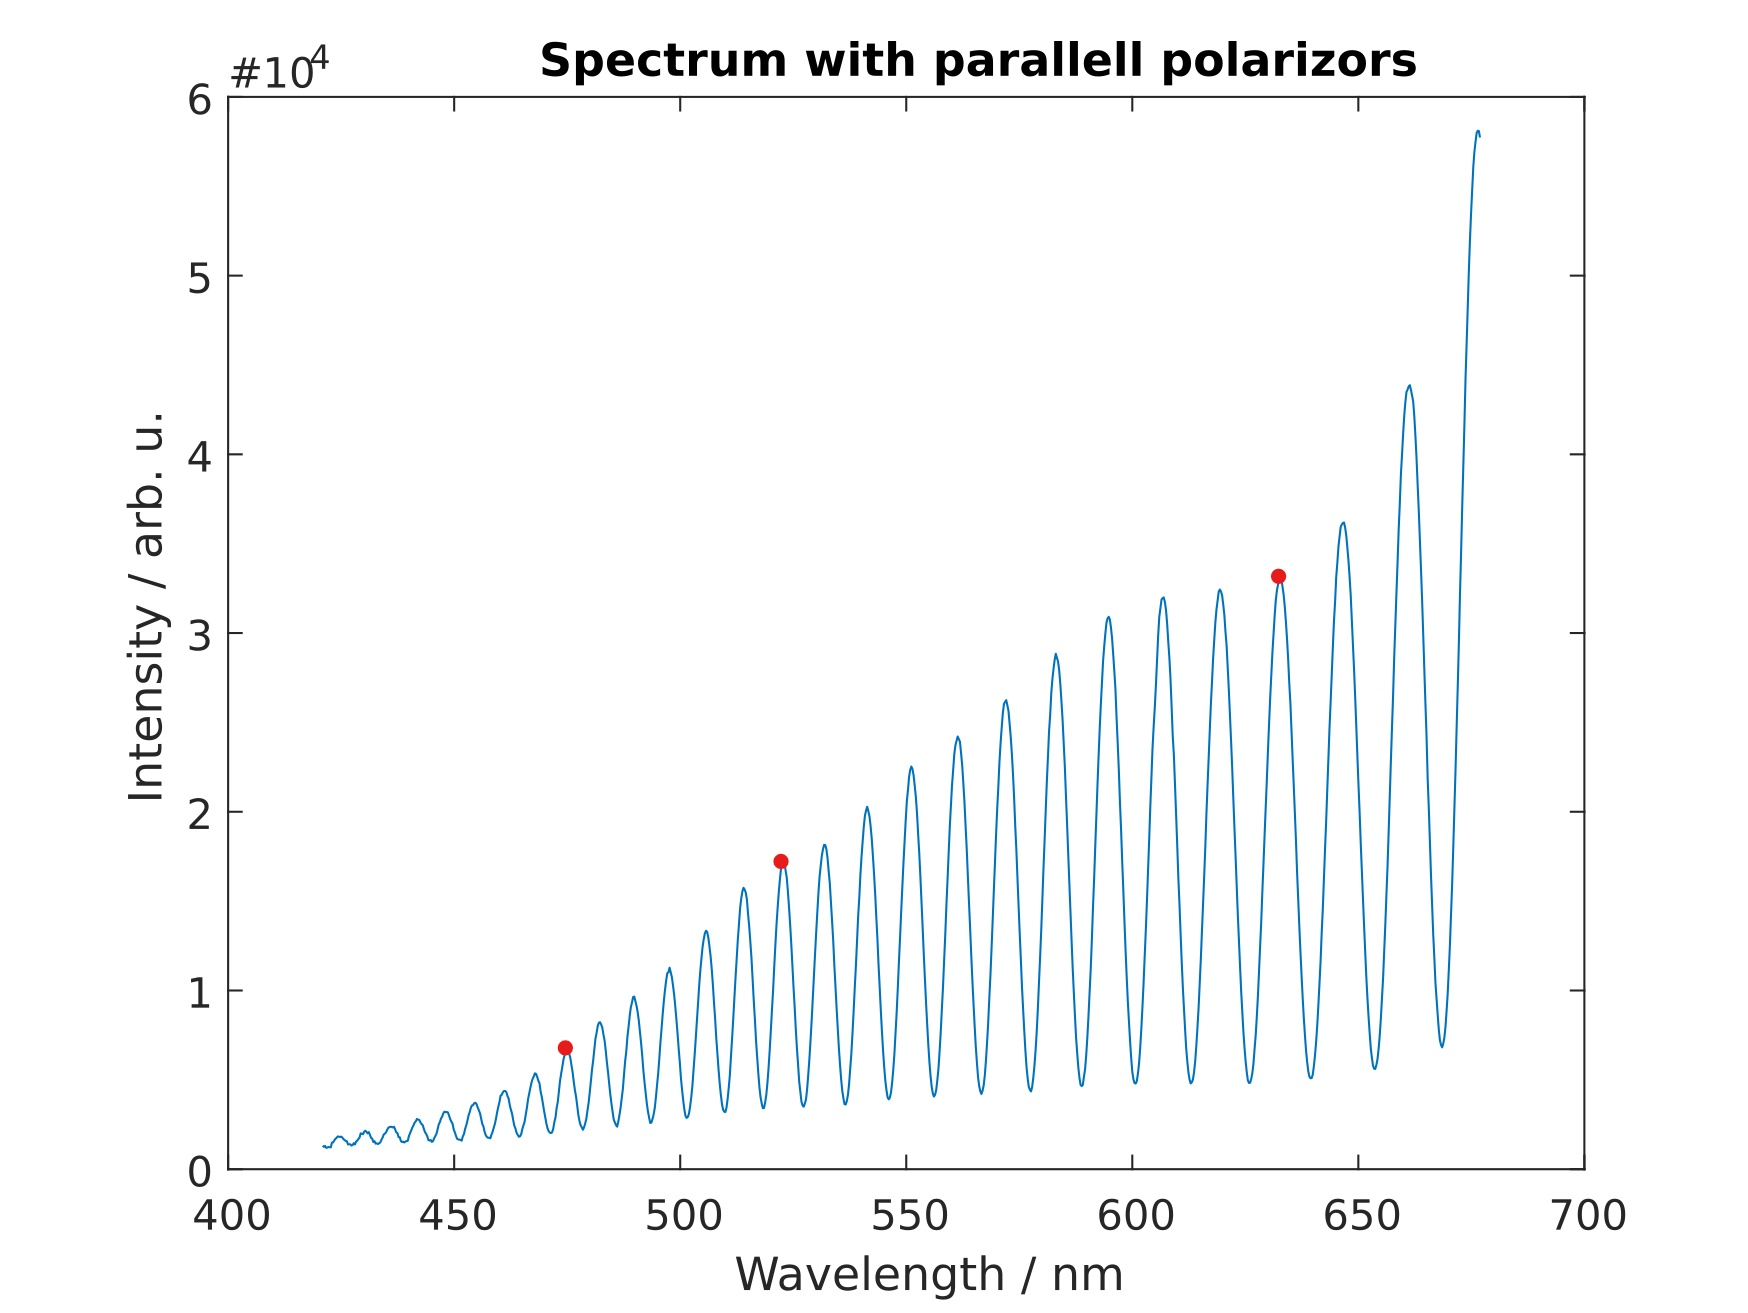
\includegraphics[width=\textwidth]{inked.jpg}
    \caption{Spectrum data for visible light. The red dots indicate which maxima where chosen for the analysis.}
    \label{fig:spectrum}
\end{figure}
Three maximas were chosen in this figure, and the wavelengths were measured, $\lambda_1$ was the first chosen maximum, $\lambda_2$ the second, $p$ maximas away from the first and
$\lambda_3$ the third, $q$ maximas away from the first.
\begin{table}[h!]
    \centering
    \begin{tabular}{|l|l|}
    \hline
    Variable                  & Value    \\ \hline
    $\lambda_1$ & 474.9 nm \\ \hline
    $\lambda_2$ & 523.1 nm \\ \hline
    $\lambda_3$ & 632.7 nm \\ \hline
    p                         & 6        \\ \hline
    q                         & 16       \\ \hline
    \end{tabular}
\end{table}
The difference in refractive index $\Delta n = n_e - n_o$ is given by Cauchys formula, equation \ref{eq:cauchy}. Combining this with the criterium for maximum for the crystal gave us a system
of equations, \ref{eq:system}.
\begin{equation}
    \Delta n(\lambda) = A + \frac{B}{\lambda^2}
    \label{eq:cauchy}
\end{equation}
\begin{align}
\begin{split}
    d(A + \frac{B}{\lambda_1^2}) = (2m + 1)\frac{\lambda_1}{2} \\
    d(A + \frac{B}{\lambda_2^2}) = (2(m-p) + 1)\frac{\lambda_2}{2} \\
    d(A + \frac{B}{\lambda_3^2}) = (2(m-q) + 1)\frac{\lambda_3}{2}
    \label{eq:system}
\end{split}
\end{align}
This system, with three unknowns ($A$, $B$ and $m$), was solved using MATLAB's \texttt{fsolve} function. 
$A$ and $B$ were plugged into the $\Delta n(\lambda)$ function, equation \ref{eq:cauchy}, and the function was plotted for the
visible wavelengths. The result is shown in figure \ref{fig:result}.
\begin{figure}[h!]
    \centering
    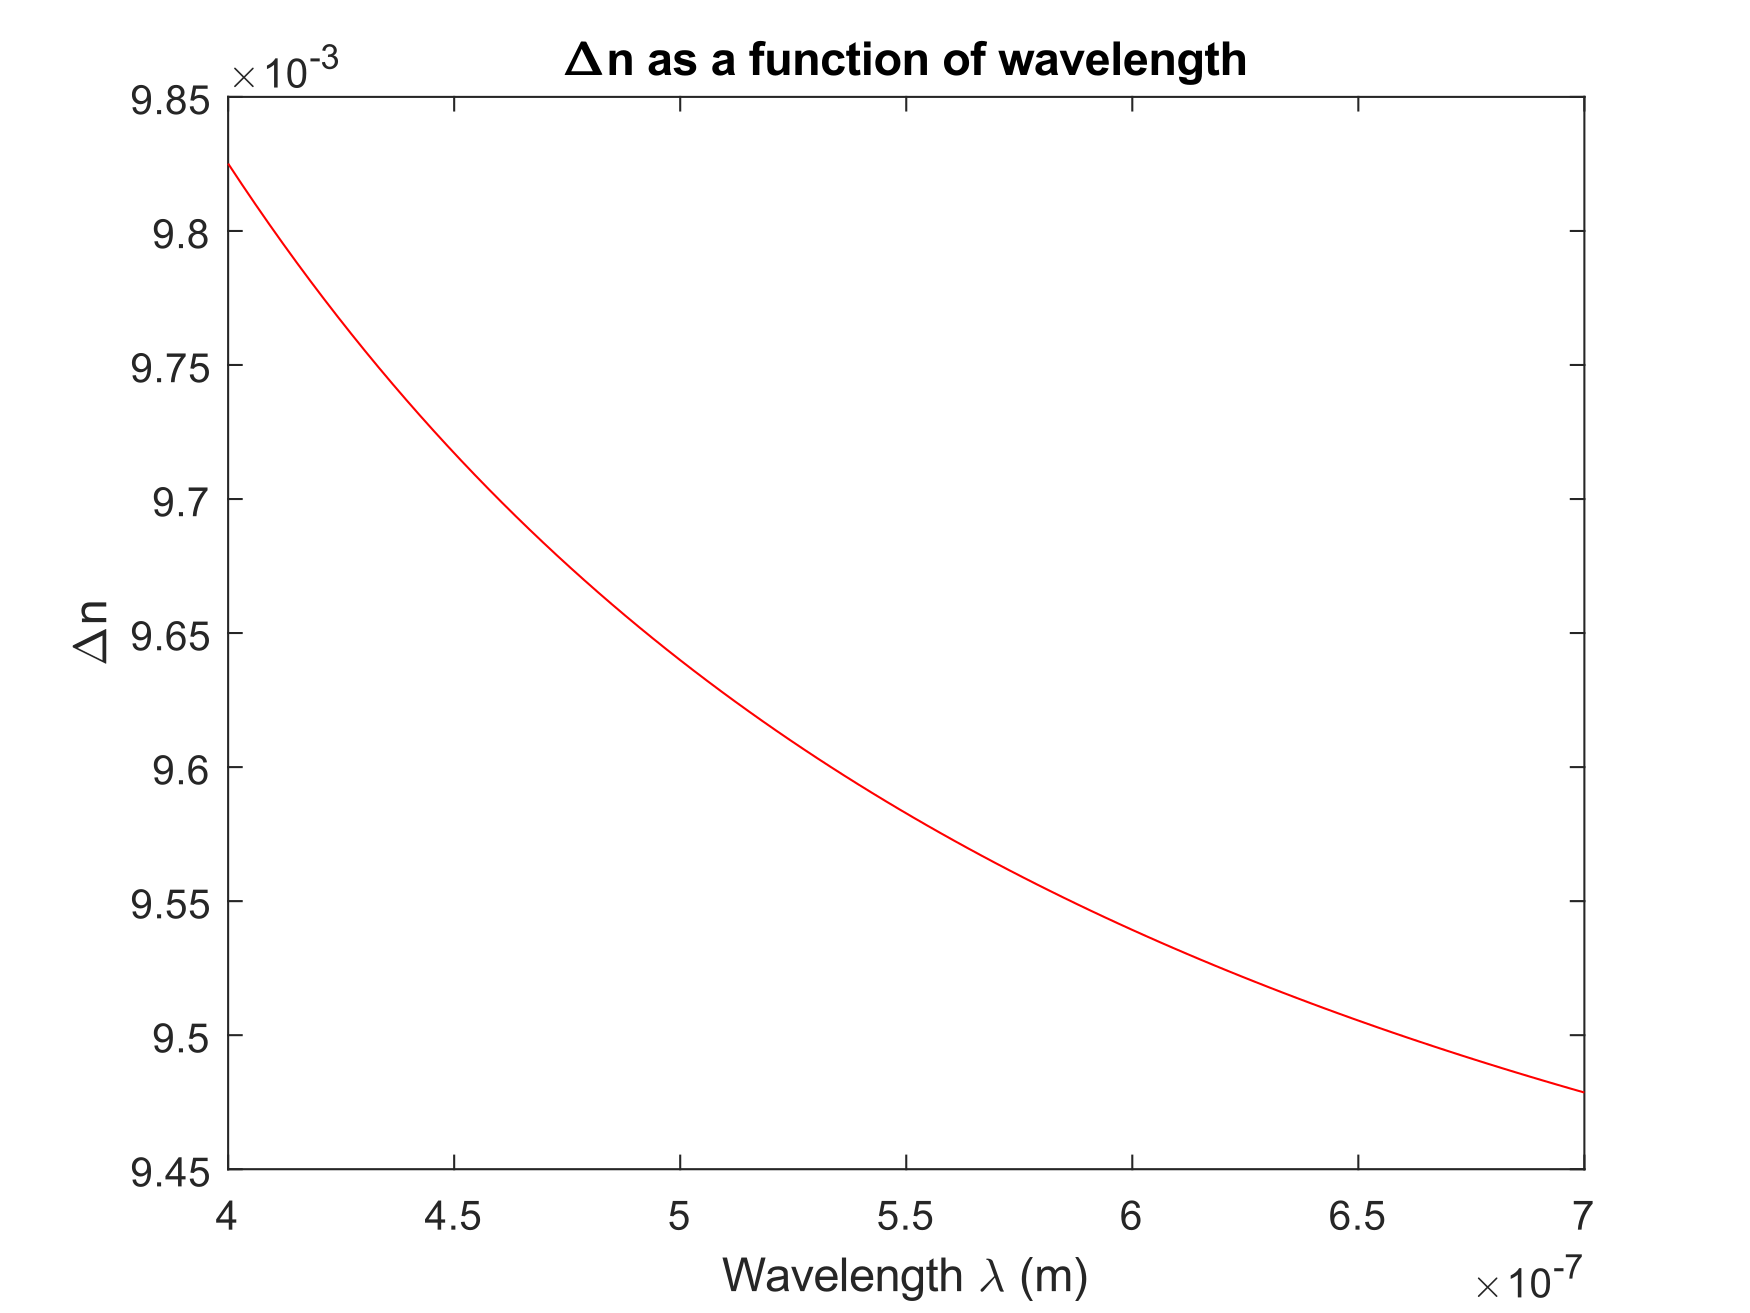
\includegraphics[width=0.7\textwidth]{result.png}
    \caption{The resulting function}
    \label{fig:result}
\end{figure}
The table value for $\Delta n$ at $\lambda = \SI{590}{\nano\meter}$ is $0.009$\cite{wiki}, and in comparison the values acquired from the experiment seem reasonable.
The difference in values can be attributed to the simple model used for the wavelength dependence of the refraction index.

\begin{thebibliography}{1}
    \bibitem{wiki}
    Wikipedia. Birefringence. Accessed 2020-05-12. Available at \url{https://en.wikipedia.org/wiki/Birefringence}
\end{thebibliography}
\end{document}